\documentclass[a4paper,11pt,report]{scrartcl}
\usepackage[dutch]{babel}
\usepackage[T1]{fontenc}
\usepackage[utf8]{inputenc}
\usepackage{lmodern}
\usepackage{amssymb}
\usepackage{color}
\usepackage{graphicx}
\usepackage{mathtools}
\DeclareGraphicsExtensions{.pdf,.png,.jpg}
\newcommand{\tab}{\hspace*{2em}}

\title{\huge\textbf{Deliverable 4}}
\subtitle{\textbf{TI2206 Software Engineering Methods\\
Delft University of Technology\\
The Netherlands}}
\author{Piet van Agtmaal 4321278\\
	    Jochem Heijltjes 1534041\\
		Arthur Hovanesyan 4322711\\
		Paul Bakker 4326091\\
		Jente Hidskes 4335732
	   }


\begin{document}
\begin{titlepage}
\maketitle
\thispagestyle{empty} %geen page numbering op opening pagina
\end{titlepage}

\newpage\section{Preamble}

The document you are currently reading is the report for deliverable four of group 21.\\

Group 21 consists of the members 
Piet van Agtmaal, Jochem Heijltjes, Arthur Hovanesyan, Paul Bakker and Jente Hidskes.\\
We are five Computer Science students at the Delft University of Technology,
The Netherlands. We created a clone of the original 2048 game for the course
Software Engineering Methods.\\

The goal of this course is to teach us how to develop software by applying the most appropriate software engineering practices, given the context of development.\\
We were asked to make a clone of the game 2048, then apply several design strategies to it and add a few extra features. This report covers what we have done, why and how.\\

We would like to thank our teacher Dr. Bachelli and our Teaching Assistants Moritz Beller and Aimee Ferouge for guiding us through this project.\\

Thank you for taking interest in this report. We hope you will enjoy reading our report and playing 2048!

\newpage\section{Introduction}

2048 is a very popular game created by by Gabriele Cirulli, based on 1024 by
Veewo Studio and conceptually similar to Threes by Asher Vollmer.\\
For this project we were asked to create a clone of the game 2048 in the Object-Oriented programming language Java, so that's what we did!\\

We didn't just make a clone of the original 2048 game, we also added
multiplayer functionality, automatic solvers allowing you to play against the computer and 
undo/redo functionality. 
Now you can challenge your computer, your neighbours, your
coworkers, your kids or even the Queen of England to play a game of 2048!\\

The purpose of this report is to present how we implemented several features/techniques and explain why they were implemented.\\
This document tells you everything you need to know about our project and to get you started playing 2048. Technical aspects of the game are covered in here as well.\\

 The structure of this report is as follows. Chapter three describes how to play 2048 and all the functionalities that have been implemented. The next chapter explains how the application is tested and how quality is being ensured. Chapter five explains which extra features were added. Chapter six covers the design patterns we have newly implemented including the corresponding class and sequence diagrams. The next chapter will explain the extra design pattern we have chosen and why and how we implemented it.\\
Finally, chapter eight will conclude this report. \\

\newpage\section{How to play 2048}

This section briefly describes how to play 2048 and provides information on
the functionality it has, such as playing the game alone, or with friends and how
to use the logging features.

\subsection{Singleplayer game}
After starting the application you will see the main menu. In the main menu,
click the \texttt{Singleplayer} button to start your singleplayer game.\\

Using the arrow keys you can move the tiles on the grid. Each time two tiles with the same
number collide, the numbers are added and the two tiles merge. Your goal is to
reach the 2048 tile!\\

To return to the menu, press \texttt{Escape} any time. Don't worry,
your current game will be saved for you! (This also applies to closing the
game!).

\subsection{Multiplayer game}
The multiplayer version is identical to the singleplayer, except here you will
compete against a friend, colleague, coworker or your worst enemy over LAN or
the internet. Your opponent does not have to be in the same room with you; they
can even be on the other side of the planet and you can still kick their
asses!\\

Your goal is to reach the 2048 tile and to get more points than your opponent.  In case you
are unable to reach the 2048 tile (because your grid is full), your opponent will either win or lose if they have more points. 

In case your grid is full, you will need to wait for your opponent to make the last move on their grid.\\

We will now briefly explain how to connect to eachother. Please refer to the
documentation of your networking equipment or software in case you experience
networking problems.

\subsubsection{Joining a game}
To connect to another player, choose the \texttt{Join a game} option in the
\texttt{Multiplayer} menu. The application will try to connect to the remote address you
entered, on port 2048, using TCP.\\
Make sure your opponent starts hosting before you try to connect or your connection attempt will fail.

\subsubsection{Hosting a game}
To have another player connect to you, choose the \texttt{Host a game} option
in the \texttt{Multiplayer} menu. The application will bind to port 2048/TCP on all the
system's network interfaces. In case you wish to play over the internet,
please make sure connections on this port are forwarded to your local address
on your NAT device. Consult the manual of your network products for more 
information.


\subsection{Challenging your computer}

You can now challenge and play against your computer. After starting the game, you will see the main menu. In the main menu, pick the \texttt{Challenge me!} option. In the next menu you can select the difficulty you want to play on.\\

Depending on your selection, the computer will make moves at a timed interval. The higher the difficulty you select, the shorter the computer will wait between moves and the better calculated its movements are.\\

The solver algorithm behind the \texttt{Easy} option is able to complete about
15\% of the grids, but only one move is made after each 1.6 seconds. The same algorithm is used for the other options, but it will be more accurate when calculating a new move. The solver will solve at least 35\% of the grids with 650 milliseconds between each move with the \texttt{Extreme} option.

If either player (you or the computer) ends up with a full grid, the game will wait for the other to complete the game before finally announcing either of you winner or loser.\\

Whoever has the highest amount of points in the end wins the game.

\subsection{Logging}
The game supports several commandline arguments for logging.\\

By default, the application will log to the standard output, using the
\texttt{ALL} logging level. If enabled, however, errors will be logged to
\texttt{stderr}. The logging level can also be adjusted.\\

The supported arguments are:
\begin{verbatim}
$ jarfile.jar [logLevel] [file]
\end{verbatim}
or, otherwise:
\begin{verbatim}
$ Launcher.java [logLevel] [file]
\end{verbatim}
Both of these fields are parsed case-insensitively.\\

Two examples:
\begin{verbatim}
$ Launcher.java debug
\end{verbatim}
will run the game and log all debug and info messages. 
\begin{verbatim}
$ Launcher.java error file
\end{verbatim}
will run the game and log all debug, error and info messages to the system's
output streams (\texttt{stdout} and \texttt{stderr}) and will write them to a
new file as well.\\

Please see the corresponding section below for more information on the possible
arguments:\\

\textbf{logLevel} can be one of the following:
\begin{description}
	\item[all] logs all messages;
	\item[info] logs info messages only;
	\item[error] log error messages and info messages;
	\item[debug] log debug, error and info messages;
	\item[none] disables logging.
\end{description}

\textbf{file}

Setting the \texttt{file} flag will write all messages of the previously set
logging level to a file. By default, a new file with the format
\texttt{2048\_YYYYMMDD\_HHmmss.log} will be created, where
\texttt{YYYMMMDDD\_HHmmss} is the time of application start.

\newpage\section{Test report}

In this section we will explain how we tested our game. We will start by
explaining how often we tested our game. Afterwards, we will explain what
kinds of testing we have done. Lastly, we will present the results of the
testing procedure.

\subsection{Test frequency}
In this section we will discuss how frequently we tested our game. This is the
first iteration where we really made use of our tests. During the MVC
refactoring, our tests came in handy for regression testing. As such, the test
frequency was higher than it normally was. The only area in which we didn't test
much are the solvers, because they are hard to predict with their random
factors. (They are covered now, but not while they were being developed).

\subsection{Testing methods}
Visual tests involved actually playing the game and analyzing logging output
manually. Unit tests simply check object properties with certain input.

Visual testing was used a lot this sprint when developing the solvers. This is
partly because of their randomness, but also because visual testing is just
plain easier here: when the static evaluation function changed, it's just easier
to run the game and look at the output rather than having to change the unit test and
then discovering the random factor is causing your test to fail. Also, a complex
piece of code such as the solver is not really testable with unit testing and
therefore, we mostly resorted to visual testing.

\subsection{Test results}
EclEmma is the tool we used for analyzing and measuring our test coverage.
As before, we analyzed our entire project using three different metrics: line,
branch and instruction coverage.\\

The results are as follows:
\begin{description}
	\item Line coverage: 77.7\%
	\item Branch coverage: 71.7\%
	\item Instruction coverage: 75.4\%
\end{description}
As with previous deliverables, we faced the same issues with code that requires
graphically rendering our game. 

\subsection{Conclusion}
The Model View Controller actually allowed us to test some code that was
previously untestable, so our coverage has again increased.

As always, we are confident our code is sufficiently tested.

\newpage\section{Exercise 1 - 20-Time}
In this section we will describe the extra features we have implemented.

We implemented the following extra features:
\begin{description}
	\item An AI that automatically solves the grid;
	\item The possibility to play against the computer;
	\item The option to ask the AI for a hint in singleplayer mode;
	\item Undo and redo functionality.
\end{description}

We chose to implement an AI feature, because the idea seemed challenging to us.
Two members of our team tried to implement their own algorithm. One mimics the
"human strategy", which basically is to keep one corner populated and move
everything into it. The other is based on the expectimax algorithm with a more
complicated static evaluation function. This second solver is not entirely
finished, because it only sporadically wins a game.\\

Both are included in the production code, however. The second solver is the only
one capable of giving the player a fair hint, because it is not tied to one
fixed corner. The other solver is capable of solving at least 35\% of the grids
and as such, is used to solve the grid in singleplayer mode and to act as
opponent when playing against the computer.\\

The undo and redo functionality is part of the singleplayer mode to give the
player the opportunity to correct mistakes when trying to solve the game. We
chose to implement this feature because one of our team members likes this
feature on the original game and he's unable to solve any puzzle without it.

The undo and redo functionality were implemented after implementing the command
pattern, so for the design documents please skip ahead. There are no design
documents for the AI.\\

The requirements that we haven't met this sprint are the win-rate of 50\% for
the AI and the possibility of letting the AI decide where to place the new tiles
after a valid move. The AI turned out to be even more complicated than expected,
so it cost us more time to get to where we are now than we anticipated. If
possible, we will continue the development into the next sprint.

\newpage\section{Exercise 2 - Design patterns}
In this section we will discuss the two chosen design patterns. Per pattern,
we will provide (in natural language) a description of why and how the pattern
is implemented, together with a class- and sequence diagram.

\subsection{The Command pattern}
The Command pattern is implemented because it made a lot of sense to do the grid 
movements through commands. If possible, it will also be used to add a
new tile to the grid randomly or via the Solver.\\

Another reason to implement the Command pattern was because we wanted to undo and redo the
movements made by the player.

\subsubsection{The implementation}
The \texttt{Command} class is an abstract class, because there are pieces of
code that every command would have to define. The invoker of a command is the
\texttt{InputHandler} class. It will invoke the class' method using the abstract
\texttt{execute()} method. We have made a \texttt{Command} class for every direction of
movement for the grid. These \texttt{Command} classes have as a receiver the
\texttt{TileHandler} class, because that performs the actual actions
of moving the tiles in the grid.\\

We have also made a \texttt{Command} class for undo and another for redo. These
commands have as a receiver: the \texttt{Grid} ,which they operate on. The \texttt{Grid} class
keeps two stacks of strings: one stack keeps track of the previous grid and the other stack 
keeps track of the grid before an undo command is executed. 
The undo and redo commands pop a string of the correct
stack and set it as the current grid. This is all done in their own implementation
of the abstract \texttt{execute()} method.

\newpage
\subsubsection{The class- and sequence diagram}
\textbf{The class diagram:}\\
\centerline{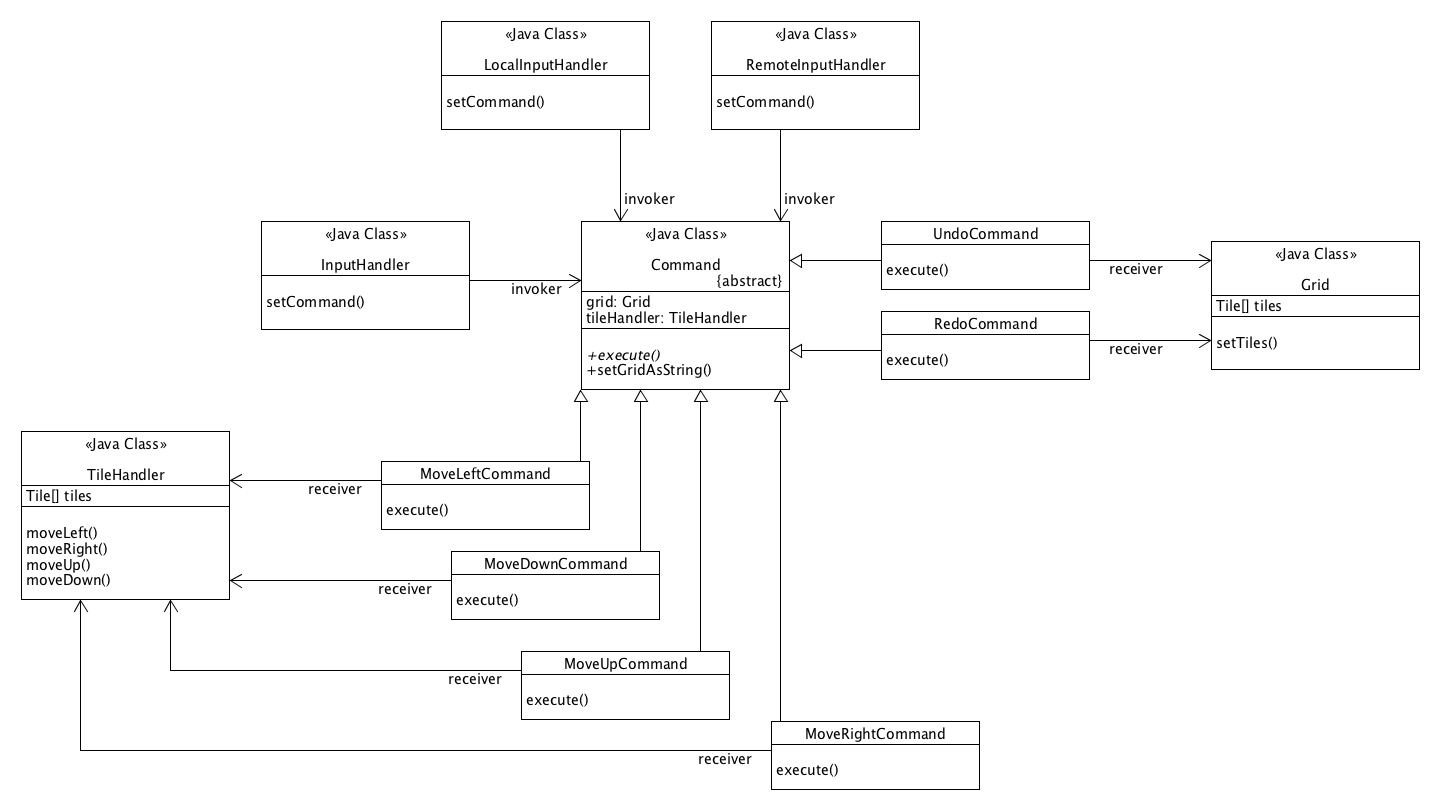
\includegraphics[scale=0.4]{sources/commandPatternUML}}

\newpage\textbf{The sequence diagram:}\\
\centerline{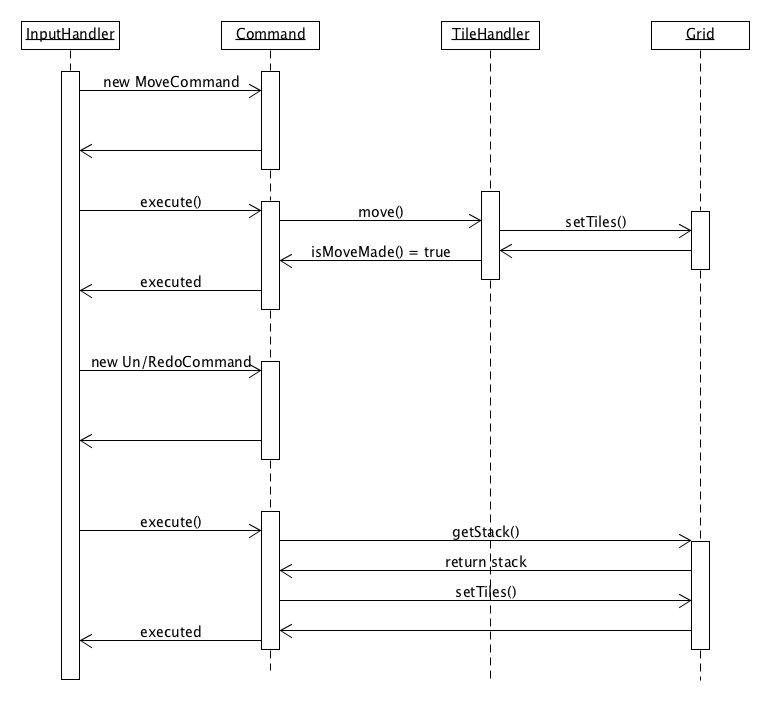
\includegraphics[scale=0.5]{sources/commandPatternSequence}}

\newpage\subsection{The State pattern}
Before the implementation, the game had different states that were defined and 

set in the TwentyFourtyGame class. This responsibility did not entirely belong 
inside this class and it was cumbersome to work with; for example, having the
opponent wait while his grid is full was impossible.\\

By implementing the state pattern we reduced duplicated code and 
made our states a lot more flexible. Since they are now their own classes, we 
can easily define state-specific behaviour, making our game not only easier to
maintain but als opening the door for future changes.

\subsubsection{The implementation}

The existing states have been replaced with classes that implement the GameState interface.
Because of this, we can dynamically set the current state through polymorphism.
Different game modes have different states and conditions for a state change. To handle this,
the GameState interface contains two update-methods that differ by their arguments:
one is used for the singleplayer mode, while the other is used for the multiplayer modes.\\

In the state class we can then look at the game's grid and change states if needed.\\

If a condition is met, we add a new screen to the ScreenStack and set the current state to the needed one.

\newpage\subsubsection{The class- and sequence diagram}
\textbf{The class diagram:}\\
\centerline{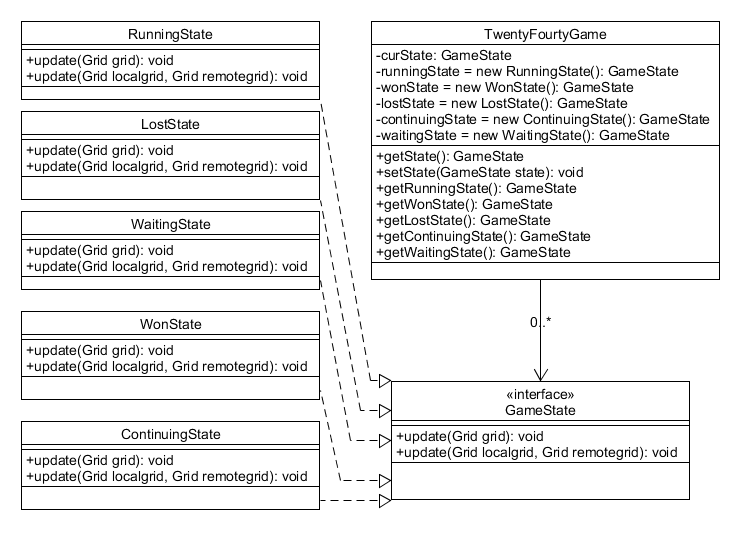
\includegraphics[scale=0.7]{sources/statePatternUML}}

\newpage\textbf{The sequence diagram:}\\
\centerline{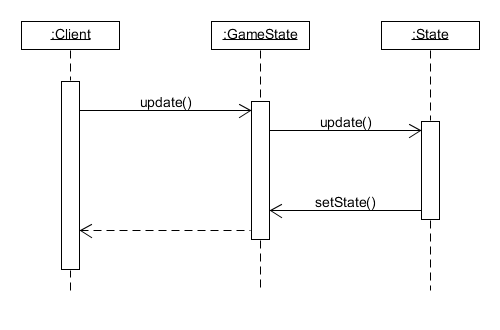
\includegraphics[scale=1]{sources/statePatternSequence}}

\newpage\section{Exercise 3 - One more design pattern}
\subsection{The MVC pattern}
We like clear structure in our code. One way to improve this was to use MVC, so
we chose MVC as extra design pattern to implement. Another reason for
implementing MVC was that it would be beneficial to the AI and it could possibly
improve our testing coverage by making more things testable on (the headless)
Devhub.

\subsubsection{The implementation}
Basically, we just split our \texttt{Grid} and \texttt{Tile} classes into
\texttt{Grid}, \texttt{DrawableGrid}, \texttt{Tile} and \texttt{DrawableTile}.\\

The \texttt{Grid} and \texttt{Tile} classes are now \texttt{Observable} and
notify the \texttt{DrawableTile} and \texttt{Scores} classes when they have
changed. The \texttt{DrawableGrid} class is merely a container class for the
\texttt{DrawableTile} instances and is also responsible for drawing the grid in
the screen.\\

\newpage\subsubsection{The class- and sequence diagram}
\textbf{The class diagram:}\\
\centerline{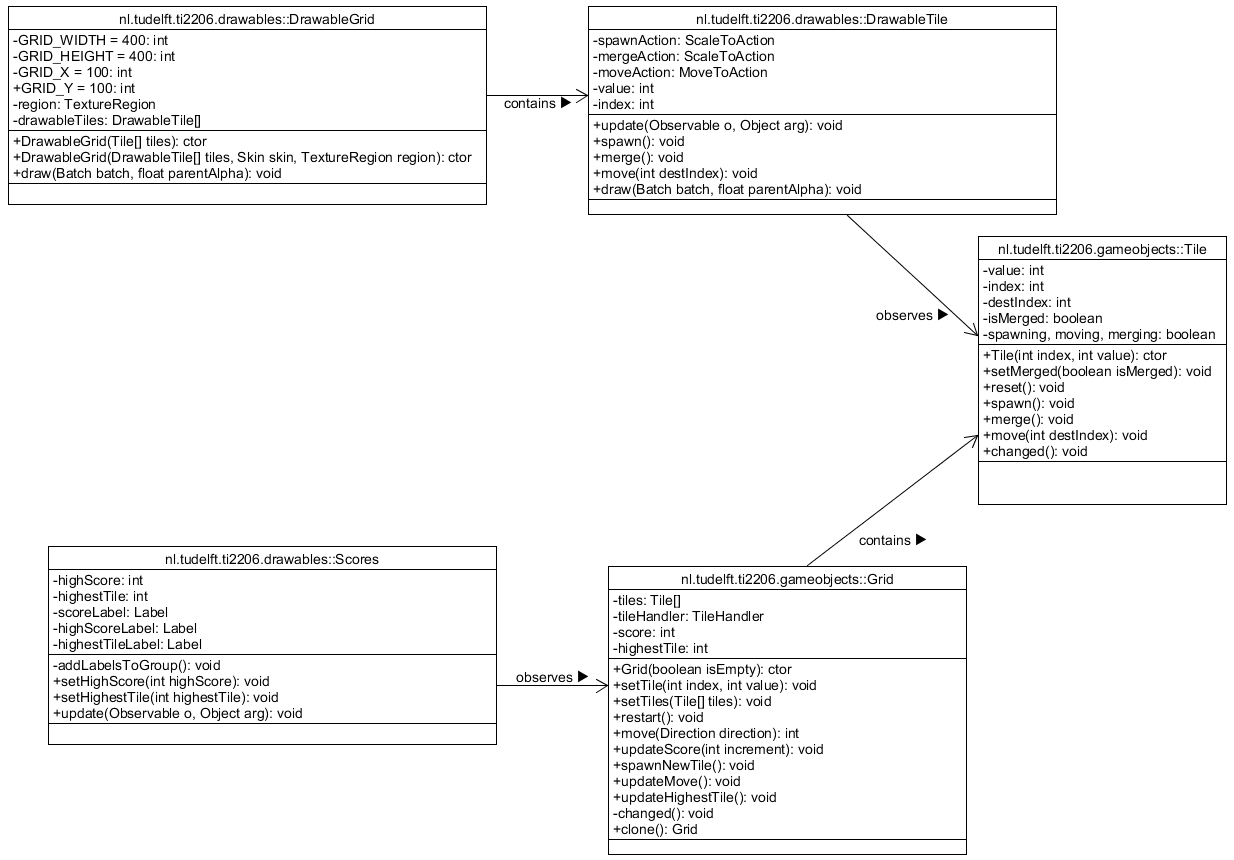
\includegraphics[scale=0.7]{sources/mvcPattern}}

\newpage\textbf{The sequence diagram:}\\
\centerline{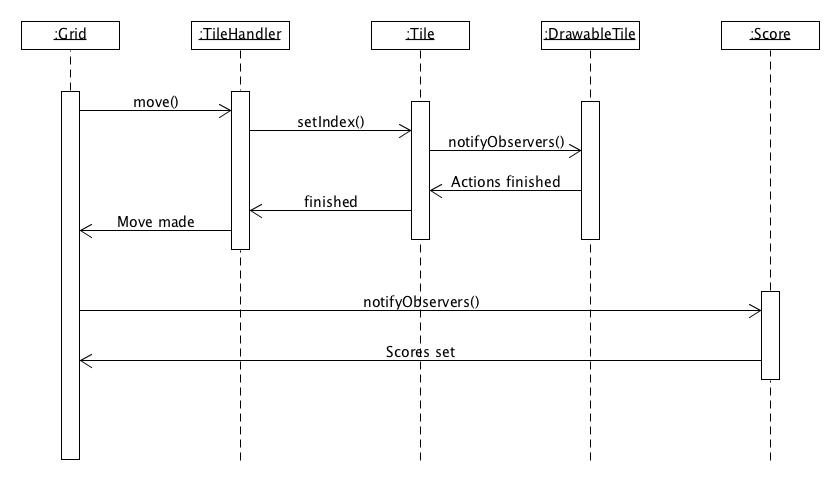
\includegraphics[scale=0.7]{sources/MVCPatternsequence}}

\newpage\section{Conclusion}

The goal of this report was to explain how we developed our 2048 clone and how
and why we implemented several features. 
The development of the game was shown to have been undertaken in several consecutive steps. First of all we created just a fully working clone of the original 2048 game. Then, we implemented a multiplayer mode where the player can play against others over the network. After that we refactored our entire game and implemented several design patterns and added several extra features we thought of ourselves.

The three extra features we implemented were:\\
- An artificial intelligence that can solve games by itself;\\
- Playing against the computer via this AI;\\
- Undo and redo functionality\\

The latest design patterns we have implemented are the command pattern, the
state pattern and the MVC (Model-View-Controller) pattern.\\

We hope you enjoyed reading this report. Have fun playing 2048!\\

\end{document}
